\chapter{Computations (Extended Attribute Evaluation with Functions and Procedures )}\indexmain{computations}\indexmain{functions}\indexmain{procedures}\indexmain{attribute evaluation}
\label{cha:computations}

In this chapter we'll have a look at the \emph{statements} of the \emph{computations} available in the rule language.
The \emph{computations} are the superordinate concept, they consist of side-effect free \emph{expressions}, and side-effect causing \emph{statements}.
Their corresponding abstractions are the \emph{functions} free of externally visible side-effects, defining an expression drop-in replacement, and the \emph{procedures} that can only be employed from statement context, defining a statement drop-in replacement; we'll visit those abstractions at the end of this chapter.

The most important task of the computations is the \emph{attribute assignment} or evaluation, assigning new values to graph element attributes.
Besides this, further types of assignments are available, and several control flow constructs as known from imperative programming languages of the C-family.
Furthermore, container methods may be called (more on this in the following chapter \ref{cha:container}), 
and global graph functions may be called (more on this in the following chapter \ref{cha:graph}).

An example implementing \indexed{depth-first search} and \indexed{breadth-first search} as computations of the rule language can be found in \texttt{test/should\_pass}, in \texttt{/DfsBfsSearch.grg}; you may have a look at the \verb#/computations_*.grg# files in that folder for further (but fabricated) examples.

\begin{rail}
  Statement:
      Assignment
    | CompoundAssignment
    | IndexedAssignment
    | VisitedAssignment
    | LocalVariableDecl
    | ContainerMethodCall
    | ProcedureCall
    | EmbeddedExec
    | Decision
    | WhileLoop
    | ForLoop
    | EarlyExit
    | ReturnStatement
    ;
\end{rail}\ixnterm{Statement}\label{computationstatemet}

%explain method calls, function calls, compound assignment, for loops in the container and graph chapters.
%The \emph{Assignment} will be explained below, the \emph{CompoundAssignment}, \emph{VisitedAssignment} and \emph{ContainerMethodCall} clauses will be introduced in chapter \ref{cha:container} and \ref{cha:graph}.


%%%%%%%%%%%%%%%%%%%%%%%%%%%%%%%%%%%%%%%%%%%%%%%%%%%%%%%%%%%%%%%%%%%%%%%%%%%%%%%%%%%%%%%%%%%%%%%%
\section{Assignments} \label{sub:assignments}\indexmain{assignments}

\begin{rail}
  Assignment:
	  NodeOrEdge '.' Ident '=' Expression ';' |
	  '::' GlobalVarIdent '.' Ident '=' Expression ';' |
	  Variable '=' Expression ';' |
	  '::' GlobalVarIdent '=' Expression ';'
	;
\end{rail}\indexmain{attribute evaluation}\ixnterm{Assignment}

Evaluation statements have \indexedsee{imperative}{attribute evaluation} semantics.
In particular, \GrG\ does not care about data dependencies (You must care for them! The assignments are just executed one after the other.).
Assignment is carried out using value semantics, even for entities of container or \texttt{string} type.
The only exception is the type \texttt{object}, there reference semantics is used.
You can find out about the available \emph{Expression}s in chapter \ref{cha:typeexpr}.

%compound assignments are given in following chapters

%%%%%%%%%%%%%%%%%%%%%%%%%%%%%%%%%%%%%%%%%%%%%%%%%%%%%%%%%%%%%%%%%%%%%%%%%%%%%%%%%%%%%%%%%%%%%%%%
\section{Local Variable Declarations} 

\begin{rail} 
  LocalVariableDecl: 
	'def' Name ':' Type ('=' Expression)? ';' |
	'def' '-' Name ':' Type '->' ('=' Expression)? ';' |
	'def' 'var' Name ':' Type ('=' Expression)? ';' |
	'def' 'ref' Name ':' Type ('=' Expression)? ';'
	;
\end{rail}\ixnterm{LocalVariableDecl}

Local variables can be defined with the syntax known for local def pattern variables, as already introduced in \ref{sec:localvarorderedevalyield}, i.e. \texttt{def var name:type} for elementary variables, or \texttt{def ref name:type} for container variables, or \texttt{def name:type} for nodes, or \texttt{def -name:type->} for edges.
At their definition, an initializing expression may be given.


%%%%%%%%%%%%%%%%%%%%%%%%%%%%%%%%%%%%%%%%%%%%%%%%%%%%%%%%%%%%%%%%%%%%%%%%%%%%%%%%%%%%%%%%%%%%%%%%
\section{Control flow} \label{sub:controlflow}\indexmain{controlflow}

Based on the value of a boolean expression different computations can be executed conditionally with the \texttt{if} and \texttt{else} statements. Please not that the braces are mandatory.

\begin{rail} 
  Decision: IfPart ((ElseIfPart)*()) (ElsePart)? ;
	IfPart: 'if' '(' BoolExpr ')' lbrace (Statement*) rbrace ;
	ElseIfPart: 'else' 'if' '(' BoolExpr ')' lbrace (Statement*) rbrace ;
	ElsePart: 'else' lbrace (Statement*) rbrace ;
\end{rail}\ixnterm{Decision}\ixkeyw{if}\ixkeyw{else}

Computations may be executed repeatedly by the \texttt{while} and \texttt{do-while} statements. Please note that the braces are mandatory and that the \texttt{do-while} loop comes without a terminating semicolon.

\begin{rail} 
  WhileLoop: 
	'while' '(' BoolExpr ')' lbrace (Statement*) rbrace |
	'do' lbrace (Statement*) rbrace 'while' '(' BoolExpr ')' 
	;
\end{rail}\ixnterm{Loop}\ixkeyw{while}\ixkeyw{do}

%\section{Container iteration}

The containers introduced in chapter \ref{cha:container} may be iterated over with a for loop, one assigning the current value to a variable, the other assigning the current index and the current value to a variable.
\begin{rail}
  ForLoop: (ForHeader | IndexedForHeader) lbrace (Statement*) rbrace;
  ForHeader: 'for' '(' Var ':' Type 'in' ContainerVar ')';
  IndexedForHeader: 'for' '(' IndexVar ':' Type '->' Var ':' Type 'in' ContainerVar ')' ;
\end{rail}\ixkeyw{in}\ixkeyw{for}\ixnterm{ForLoop}

Loop body execution may be exited early or continued with the next iteration with the \texttt{break} and \texttt{continue} statements. Such a statement must not occur outside of a loop.

\begin{rail} 
  EarlyExit: 
	'break' ';' |	'continue' ';'
	;
\end{rail}\ixnterm{EarlyExit}\ixkeyw{break}\ixkeyw{continue}


%%%%%%%%%%%%%%%%%%%%%%%%%%%%%%%%%%%%%%%%%%%%%%%%%%%%%%%%%%%%%%%%%%%%%%%%%%%%%%%%%%%%%%%%%%%%%%%%
\section{Embedded Exec} 

As in the rules (cf. chapter \ref{cha:imperativeandstate}), \texttt{exec} statements may be embedded.
They are executing the graph rewrite sequence (see chapter \ref{cha:xgrs}) contained, with access to the variables defined outside.
This means for one reading this variables, but for the other assigning to that variables with \texttt{yield}.
The embedded \texttt{exec}s allow to apply rules from the computations, more exactly: from the procedures (embedded execs are not available in functions), while the sequence computations (cf. \ref{sec:seqcomp}) may call defined computations (functions in expression context, and procedures in statement context), mixing and merging declarative rule-based graph rewriting (pattern matching and dependent modifications) with traditional graph programming.
This construct achieves a further step in the direction of blending rule-based with traditional programming; the main step is the extension of the attribute assignments, the only statement available in the original {\scshape GrGen}, into the full-fledged computations pictured in this and the following chapters.

\begin{description}
\item[\texttt{exec(.)}] executes the graph rewrite sequence given. 
\end{description}



%%%%%%%%%%%%%%%%%%%%%%%%%%%%%%%%%%%%%%%%%%%%%%%%%%%%%%%%%%%%%%%%%%%%%%%%%%%%%%%%%%%%%%%%%%%%%%%%
\section{Computation Definition and Call} \label{sub:compdef}\indexmain{computation definition}

Computations that are occuring frequently may be factored out into a computation definition given in the header of a rule file.
Such compound computations can be built and abstracted into reusable entities in two different forms, \emph{functions} usable(/callable) from expression context, and \emph{procedures} usable(/callable) from statement context.
Besides, several built-in functions and procedures are available, ready to be called and reused with the same syntax.
(Furthermore, external functions and computations may be declared, callable with the same syntax, too.)

%-----------------------------------------------------------------------------------------------
\subsection{Function Definition and Call}\label{sub:functions}\label{sec:funccall} 

Functions return exactly one output value, and can thus be used from the expressions with their compositional semantics.
They are side-effect free, meaning they are not allowed to change the graph while being executed ---
so you are not allowed to call procedures (self-defined as well as built-in) from with a function definition.
On the other hand we consider pure functional programming not a help but a burden, so you are free to declare local variables and assign them as you like inside the function definitions; they only must behave as functions at the outside.

\begin{rail} 
  FunctionDefinition: 
	Name '(' Parameters ')' ':' ReturnType \\
	lbrace (Statement+) rbrace;
  Parameters: (Parameter * ',');
  Parameter: IdentDecl ':' NodeType |
  '-' IdentDecl ':' EdgeType '->' |
  ('var' | 'ref') IdentDecl ':' VarType;
\end{rail}\ixnterm{FunctionDefinition}\ixnterm{Parameter}\ixkeyw{var}\ixkeyw{ref}

The function definition must return a value with a return statement (so there must be at least one return statement).
The type of the one return value must be compatible to the return type specified in the computation definition.
(A return statement must not occur outside of a computation definition.)

\begin{rail}
  ReturnStatement: 'return' '(' Expression ')' ';' ;
\end{rail}\ixkeyw{return}\ixnterm{ReturnStatement}

\begin{rail}
  FunctionCall: Name '(' (Expression * ',') ')' ;
\end{rail}\ixnterm{FunctionCall}

A such defined function may then be called as an expression atom from anywhere in the rule language file where an expression is required; or even from the sequence computations where an expression is required.
Besides the built-in functions that are called with the same syntax;
table~\ref{funcstab} lists the built-in functions of the rule language at a glance.

%\makeatletter
\begin{table}[htbp]
\centering
\begin{tabular}{|l|}
\hline
\texttt{nodes([NodeType]):set<Node>}\\
\texttt{edges([EdgeType]):set<Edge>}\\
\hline
\texttt{source(Edge):Node}\\
\texttt{target(Edge):Node}\\
\texttt{opposite(Edge,Node):Node}\\
\hline
\texttt{adjacent(Node[,EdgeType[,NodeType]]):set<Node>}\\
\texttt{adjacentIncoming(Node[,EdgeType[,NodeType]]):set<Node>}\\
\texttt{adjacentOutgoing(Node[,EdgeType[,NodeType]]):set<Node>}\\
\texttt{incident(Node[,EdgeType[,NodeType]]):set<Edge>}\\
\texttt{incoming(Node[,EdgeType[,NodeType]]):set<Edge>}\\
\texttt{outgoing(Node[,EdgeType[,NodeType]]):set<Edge>}\\
\hline
\texttt{reachable(Node[,EdgeType[,NodeType]]):set<Node>}\\
\texttt{reachableIncoming(Node[,EdgeType[,NodeType]]):set<Node>}\\
\texttt{reachableOutgoing(Node[,EdgeType[,NodeType]]):set<Node>}\\
\texttt{reachableEdges(Node[,EdgeType[,NodeType]]):set<Edge>}\\
\texttt{reachableEdgesIncoming(Node[,EdgeType[,NodeType]]):set<Edge>}\\
\texttt{reachableEdgesOutgoing(Node[,EdgeType[,NodeType]]):set<Edge>}\\
\hline
\texttt{isAdjacent(Node,Node[,EdgeType[,NodeType]]):boolean}\\
\texttt{isAdjacentIncoming(Node,Node[,EdgeType[,NodeType]]):boolean}\\
\texttt{isAdjacentOutgoing(Node,Node[,EdgeType[,NodeType]]):boolean}\\
\texttt{isIncident(Node,Edge[,EdgeType[,NodeType]]):boolean}\\
\texttt{isIncoming(Node,Edge[,EdgeType[,NodeType]]):boolean}\\
\texttt{isOutgoing(Node,Edge[,EdgeType[,NodeType]]):boolean}\\
\hline
\texttt{isReachable(Node,Node[,EdgeType[,NodeType]]):boolean}\\
\texttt{isReachableIncoming(Node,Node[,EdgeType[,NodeType]]):boolean}\\
\texttt{isReachableOutgoing(Node,Node[,EdgeType[,NodeType]]):boolean}\\
\texttt{isReachableEdges(Node,Edge[,EdgeType[,NodeType]]):boolean}\\
\texttt{isReachableEdgesIncoming(Node,Edge[,EdgeType[,NodeType]]):boolean}\\
\texttt{isReachableEdgesOutgoing(Node,Edge[,EdgeType[,NodeType]]):boolean}\\
\hline
\texttt{inducedSubgraph(set<Node>):graph}\\
\texttt{definedSubgraph(set<Edge>):graph}\\
\texttt{import(string):graph}\\
\texttt{copy(graph):graph}\\
\hline
\texttt{min(Number,Number):Number}\\
\texttt{max(Number,Number):Number}\\
\texttt{abs(Number):Number}\\
\hline
\texttt{pow([double,]double):double}\\
\texttt{log(double[,double]):double}\\
\hline
\texttt{sin(double):double}\\
\texttt{cos(double):double}\\
\texttt{tan(double):double}\\
\hline
\texttt{arcsin(double):double}\\
\texttt{arccos(double):double}\\
\texttt{arctan(double):double}\\
\hline
\end{tabular}
\caption{Functions at a glance}
\label{funcstab}
\end{table}


%-----------------------------------------------------------------------------------------------
\subsection{Procedure Definition And Call}\label{sub:procedures}\label{sec:proccall} 
%You may call any of the built-in procedures that will be introduced in the following chapters or any of your defined procedures just for its side effects, throwing away the result.

Procedures may return between zero and $k$ (arbitrary, but statically fixed) output values, and are thus only callable as a statement, with (or without) a multiple-value assignment.
They are allowed to manipulate the graph as needed while being executed;
so in a procedure definition you are free to call other procedures (self-defined as well as built-in).

\begin{rail} 
  ProcedureDefinition: 
	Name '(' Parameters ')' ReturnTypes \\
	lbrace (Statement+) rbrace;
  ReturnTypes: (':' '(' (ReturnType + ',') ')' )?;
\end{rail}\ixnterm{ProcedureDefinition}\ixnterm{Parameter}\ixkeyw{var}\ixkeyw{ref}

Please note the syntactic difference distinguishing the procedures from the functions: the return types are enclosed in parenthesis (or omitted altogether).
The computation definition may return between zero and $k$ values.
It must be always ended with a return statement; the type of the return values must be compatible to the return types specified in the computation definition.
(A return statement must not occur outside of a computation definition.)

\begin{rail}
  ReturnStatement: 'return' ( '(' (Expression + ',') ')' )? ';' ;
\end{rail}\ixkeyw{return}\ixnterm{ReturnStatement}

\begin{rail}
  ProcedureCall: (OutputAssignment)? Name '(' (Expression * ',') ')' ;
  OutputAssignment: '(' (AssignmentTarget + ',') ')' '=' ;
\end{rail}\ixnterm{ProcedureCall}\ixnterm{OutputAssignment}\ixnterm{AssignmentTarget}

A such defined procedure may then be called as a statement atom from anywhere in the rule language file where an attribute evaluation (/computation) is required; or even from the sequence computations where a statement is required.
Besides the built-in procedures that are called with the same syntax;
table~\ref{procstab} lists the built-in procedures of the rule language at a glance.

Please note that the \emph{OutputAssignment} is optional, you may execute a procedure just for its side effects; this kind of call is even the most common as many built-in procedures don't return values at all but are just executed for their state changes.
The \emph{AssignmentTarget} may be any of the LHS expressions supported by the different \emph{AssignmentStatements} (a def variable, a def variable yielded to, a global variable, a graph element attribute, an indexed target, or a visited flag of a graph element), and it may be def variable that gets just declared (\emph{LocalVariableDecl}), using the procedure output for initialization.

%\makeatletter
\begin{table}[htbp]
\centering
\begin{tabular}{|l|}
\hline
\texttt{add(NodeType):(Node)}\\
\texttt{addCopy(Node):(Node)}\\
\texttt{add(EdgeType,Node,Node):(Edge)}\\
\texttt{addCopy(Edge,Node,Node):(Edge)}\\
\texttt{rem(NodeType)}\\
\texttt{rem(EdgeType)}\\
\texttt{retype(Node,NodeType):(Node)}\\
\texttt{retype(Edge,EdgeType):(Edge)}\\
\texttt{clear()}\\
\hline
\texttt{merge(Node,Node)}\\
\texttt{redirectSource(Edge,Node)}\\
\texttt{redirectTarget(Edge,Node)}\\
\texttt{redirectSourceAndTarget(Edge,Node,Node)}\\
\hline
\texttt{insert(graph)}\\
\texttt{insertCopy(graph,Node):(Node)}\\
\texttt{insertInduced(set<Node>,Node):(Node)}\\
\texttt{insertDefined(set<Edge>,Edge):(Edge)}\\
\texttt{export(string)}\\
\texttt{export(graph,string)}\\
\hline
\texttt{valloc():(int)}\\
\texttt{vfree(int)}\\
\texttt{vreset(int)}\\
\texttt{vfreenonreset(int)}\\
\hline
\texttt{startTransaction():(int)}\\
\texttt{pauseTransaction(int)}\\
\texttt{resumeTransaction(int)}\\
\texttt{commitTransaction(int)}\\
\texttt{rollbackTransaction(int)}\\
\hline
\texttt{emit(string)}\\
\texttt{record(string)}\\
\hline
\end{tabular}
\caption{Procedures at a glance}
\label{procstab}
\end{table}

\subsection{The Big Picture}
Figure \ref{figcomptypescallsuses} displays the different computation types of \GrG, and how they may use and call each other. On top the strategy language for rule control, to the left the declarative rules and subpatterns, and to the right the imperative parts for attribute computations or traditional graph programming. The statements include the expressions and non-graph changing statements.

\begin{figure}[hptb]
  \centering
  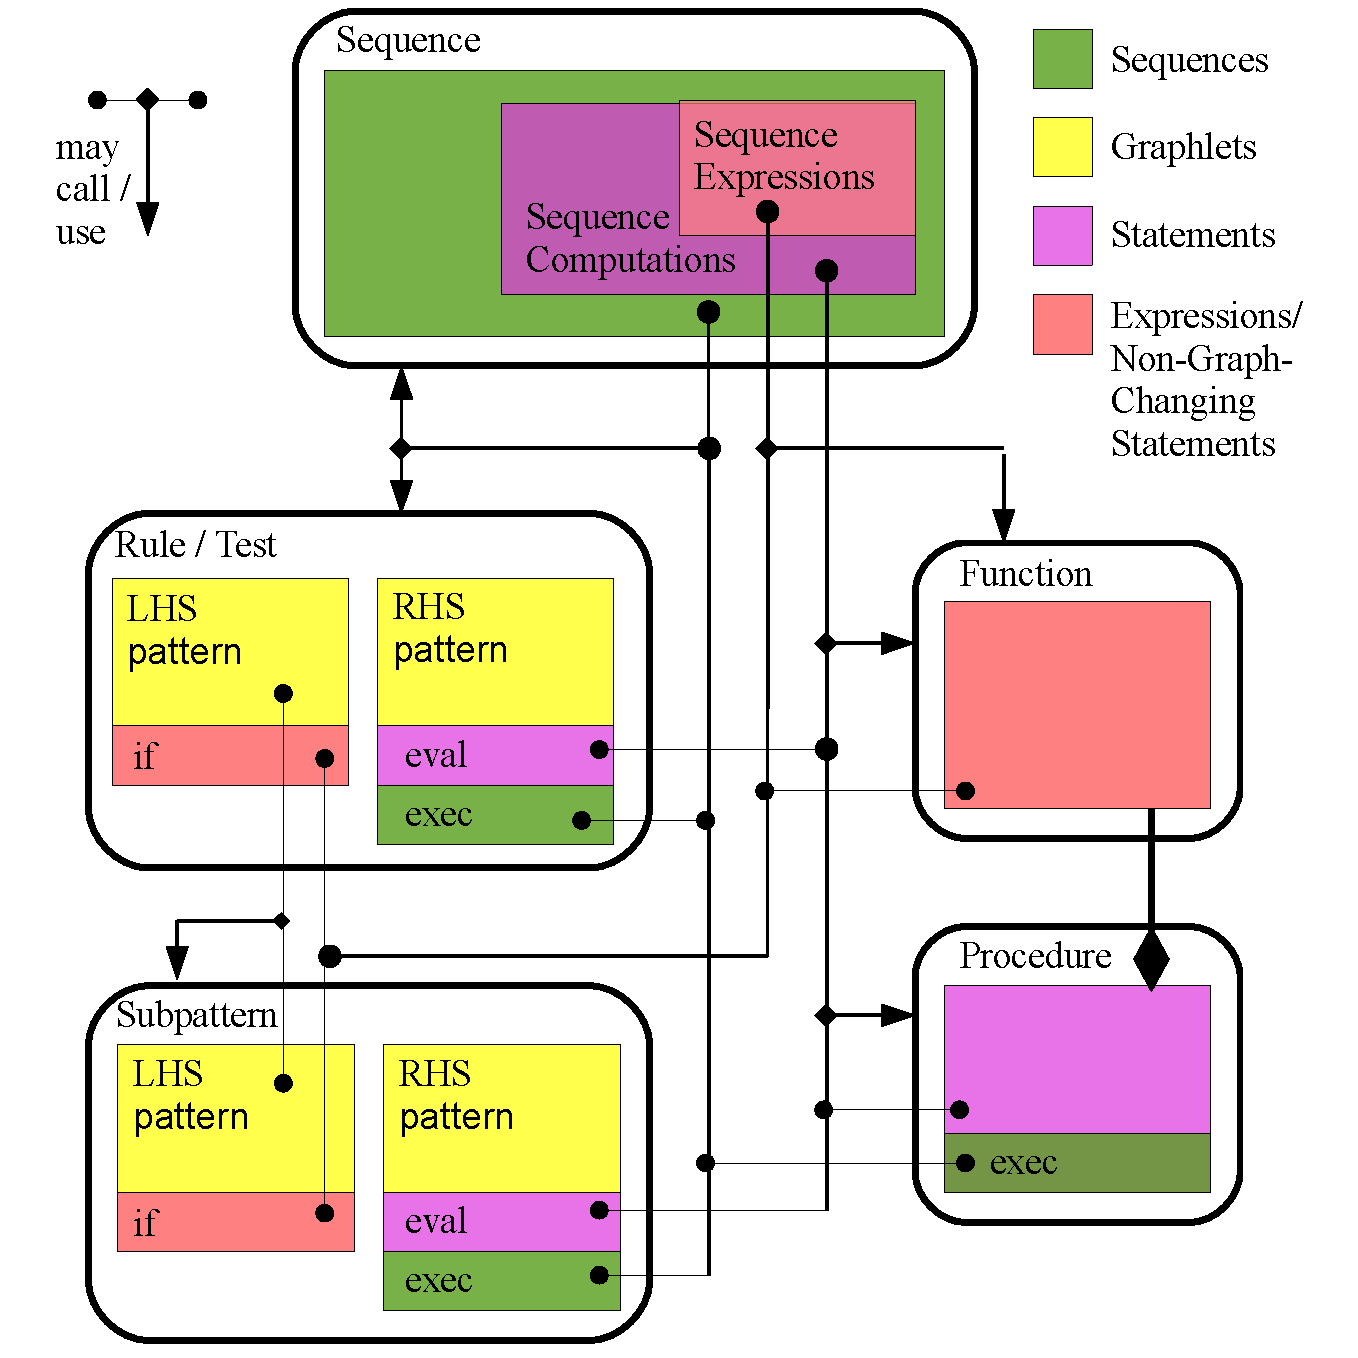
\includegraphics[width=1.0\textwidth]{fig/ComputationContainmentAndCallability}
  \caption{Computation Types and Possible Calls/Uses}
  \label{figcomptypescallsuses}
\end{figure}

